\documentclass[12pt]{report}
 
\usepackage[latin1]{inputenc}
\usepackage[T1]{fontenc}
\usepackage[francais]{babel}
\usepackage{graphicx}

\begin{document}
 
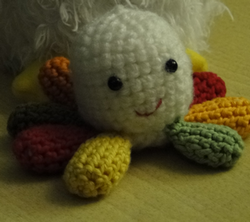
\includegraphics{ploupi.png} %faut m�tre le chemin de l'image ex:C:\Cassoulet\Documents\fichierslatex\chapitre9\poulpy.png.
\newpage
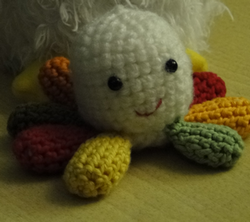
\includegraphics[width=200]{ploupi.png}
\newpage
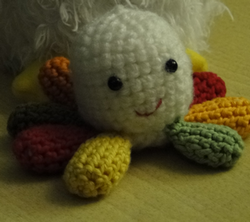
\includegraphics[height=200]{ploupi.png}
\newpage
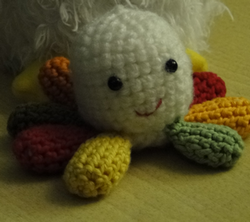
\includegraphics[height=200, width=600]{ploupi.png}  
% Ici, Poulpy est un peu plate
\newpage
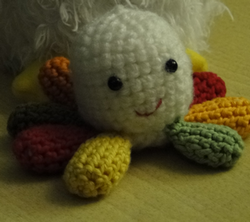
\includegraphics[scale=1.5]{ploupi.png}  
% Ici, Poulpy est plut�t grande
\newpage
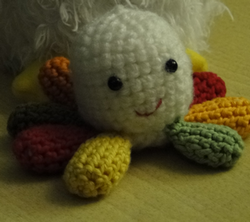
\includegraphics[angle=45]{ploupi.png} % Poulpy en biais
\newpage


%le flottant
\begin{figure} 
\begin{center}
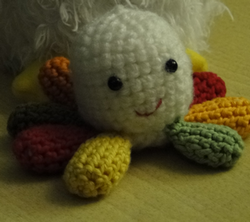
\includegraphics{ploupi.png} 
\end{center} 
\end{figure}
%fin le flottant

%\begin{figure}[les options non s�par�es par des virgules]
%Quelques d�monstrations ci-dessous. 
%Le � ! � est utilis� ici pour faire comprendre
%� LaTeX que nous insistons � �norm�ment � sur une option.
%\begin{figure}[b] %nous voulons le flottant en bas.
%\begin{figure}[!b] %nous voulons le flottant en bas (avec insistance).
%\begin{figure}[bt] %nous voulons le flottant en bas, ou en haut s'il ne peut pas�tre en bas.
%\begin{figure}[h] %nous voulons le flottant ici.
%\begin{figure}[H] %nous voulons le flottant ICI !
%\begin{figure}[hb] %nous voulons le flottant ici, ou en bas si cela n'est paspossible.

%LES L�GENDES:
\begin{figure}
\begin{center}
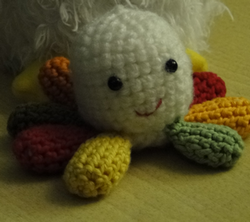
\includegraphics{ploupi.png} 
\end{center}
\caption{ploupi est multicolore}
\label{ploupi est multicolore}
\end{figure}


\end{document}
